\chapter{%
    Лабораторная работа №2\\
    Создание печатного узла согласующей цепи
}

\section{Вариант 1}

Создать печатный узел схемы согласующей цепи (Рис.~\ref{fig:matching-schematic}), выполненной на полусосредоточенных элеметах.
Использовать ёмкости $C_1 = 2.7~\text{пФ}$ и $C_2 = 0.5~\text{пФ}$ типов 0402 и 0603 соответственно.
Толщину платы и ширину микрополосковой линии взять равными $0.5~\text{мм}$.
\begin{figure}[H]
    \centering
    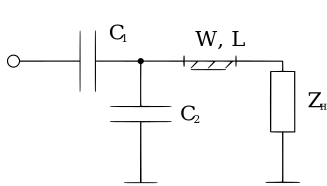
\includegraphics[width=0.6\textwidth]{matching-schematic}
    \caption{Схема согласующей цепи}%
    \label{fig:matching-schematic}
\end{figure}

\subsection{Схематический уровень}

Для выполнения поставленной задачи создадим проект, в котором соберём схему согласующей цепи (Рис.~\text{fig:matching-circuit}).
\begin{figure}[H]
    \centering
    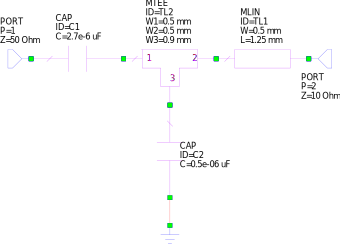
\includegraphics[width=0.6\textwidth]{matching-circuit}
    \caption{Схема согласующей цепи}%
    \label{fig:matching-circuit}
\end{figure}

\subsection{Конструкторская ячейка}

Пользуясь инструментом \textbf{Layout Manager} создадим констркуторские ячейки для обоих конденсаторов.
Результат работы представлен на рис.~\ref{fig:layout-cells}.
\begin{figure}[H]
    \centering
    \begin{subfigure}{0.45\textwidth}
        \centering
        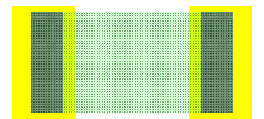
\includegraphics[width=\textwidth]{0603-layout-cell}
        \caption{}%
        \label{fig:0603-layout-cell}
    \end{subfigure}
    \hfill
    \begin{subfigure}{0.45\textwidth}
        \centering
        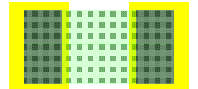
\includegraphics[width=\textwidth]{0402-layout-cell}
        \caption{}%
        \label{fig:0402-layout-cell}
    \end{subfigure}
    \caption{%
        Топологии конструкторских ячеек конденсаторов:
        (а) 0603;
        (б) 0402;
    }%
    \label{fig:layout-cells}
\end{figure}

\subsection{Топологическое представление}

Пользуясь инструментом \textbf{Layout Manager} создадим топологию проектируемой схемы.
Результат представлен на рис.~\ref{fig:matching-layout}.
\begin{figure}[H]
    \centering
    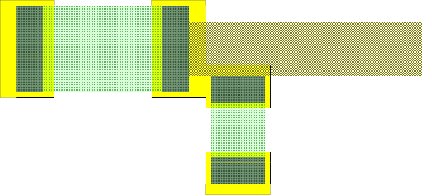
\includegraphics[width=0.7\textwidth]{matching-layout}
    \caption{Топология цепи согласования}%
    \label{fig:matching-layout}
\end{figure}
